\documentclass[12pt,twoside]{report}
\usepackage{fancyhdr}
\pagestyle{fancy}
\usepackage[utf8]{inputenc}
\usepackage{amsmath}
\usepackage{amsfonts}
\usepackage{amssymb}
\usepackage{hyperref}
\usepackage{graphicx}
\usepackage{subcaption}
\usepackage{sidecap}
\usepackage{float}
\graphicspath{{../images/}}
\begin{document}
\chapter{Dark Matter}

	For nearly a century, experimental evidence has suggested that a large portion of the universe is made up of a non-luminous type of matter.  While this dark matter has only been detected indirectly via its interaction with normal matter through the gravitational force, recent experiments conclude that approximately 26\% of the entire energy density of the universe is comprised by dark matter.

	In this chapter, I will focus on the leading dark matter model, the experimental evidence for its existence, the different candidates for particle dark matter, and the current detection methods employed in the search for particle dark matter.
	
	
\section{$\Lambda$CDM Model}

	One of the guiding principles of cosmology are the assumptions that the universe is both homogeneous and isotropic at large enoug scales (typically on the order 100 Mpc or $10^{5}$ light years).  Continuing with these principles and maintaining generality, we can arrive at the Robertson-Walker space-time metric
	\begin{equation}
		ds = -c^{2}dt^{2} + a(t)^{2}\left( \dfrac{dr^{2}}{1 - kr^{2}} + r^{2}d\Omega^{2}\right)
	\end{equation}
Here, $a(t)$ is called the \emph{scale factor}, an arbitrary function of time allowing for time dependent changes of the universe, and $k$ is a constant modeling the curvature of the universe.  For $k=-1$, the universe is considered open, for $k=1$, the universe is considered close, and at $k=0$ we are left with our Euclidean (flat) universe.  Note that for $a(t) = 1$ and $k = 0$ the Robertson-Walker metric reduces to the Minkowski metric.

	Using this metric in combination with Einstein's equation we can derive the equations for the Friedmann-Robertson-Walker universe described by the Friedmann equations.
	\begin{equation}
		\frac{\ddot{a}}{a} = -\frac{4 \pi G}{3} \left( \rho + 3p \right)
	\end{equation}
	\begin{equation}
		\left( \frac{\dot{a}}{a}\right)^{2} = \frac{8 \pi G}{3} \rho - \frac{k}{a^2}
	\end{equation}

	We can define several useful (and commonplace) parameters to simplify the second Friedmann equation further.
	\begin{description}
		\item[Hubble Parameter] $ H = \frac{\dot{a}}{a} $
		\item[Critical Density] $ \rho_{crit} = \frac{3H^2}{8 \pi G} $
		\item[Density Parameters] $ \Omega_{i} = \frac{8 \pi G}{3H^2} \rho_{i} = \frac{\rho_{i}}{\rho_{crit}} $
	\end{description}	
	
	\begin{equation}
		\Omega - 1 = \frac{k}{H^2 a^2}, \ \ \ \ \Omega = \sum_{i} \Omega_{i} = \Omega_{\Lambda} + \Omega_{CDM} + \Omega_{Baryon} + \Omega_{Rad} + \Omega_{k} \ldots 
	\end{equation}
	
	Here the critical density is defined such that the universe is flat ($k=0$) and the final density parameter is the sum of the individual density parameters.  One can think of $\frac{\Omega_i}{\Omega}$ as what part of the total matter and energy budget a particular component makes up.  The main contributors to the density of the universe are dark energy and cold dark matter hence the $\Lambda$CDM Model.  Measurements of the various density parameters and other $\Lambda$CDM parameters has been a very big area of research over the last two decades and will be discussed later in this chapter.
	
\section{Evidence of Dark Matter}

\subsection{Dynamical Constraints from Clusters of Galaxies}

The first evidence of dark matter came from Fritz Zwicky in 1933.  Zwicky used a basic application of the virial theorem on galaxies in the Coma Cluster	to estimate the mass of the cluster.  He then  estimated the total mass based on the brightness of the cluster and found significant disagreement between the results leading him to the conclusion that "if this would be confirmed we would get the surprising result that dark matter is present in much greater amount than luminous matter." (Zwicky, 1933, \href{http://www.ymambrini.com/My_World/History_files/Zwicky.pdf}{source})
	
\begin{figure}[h]
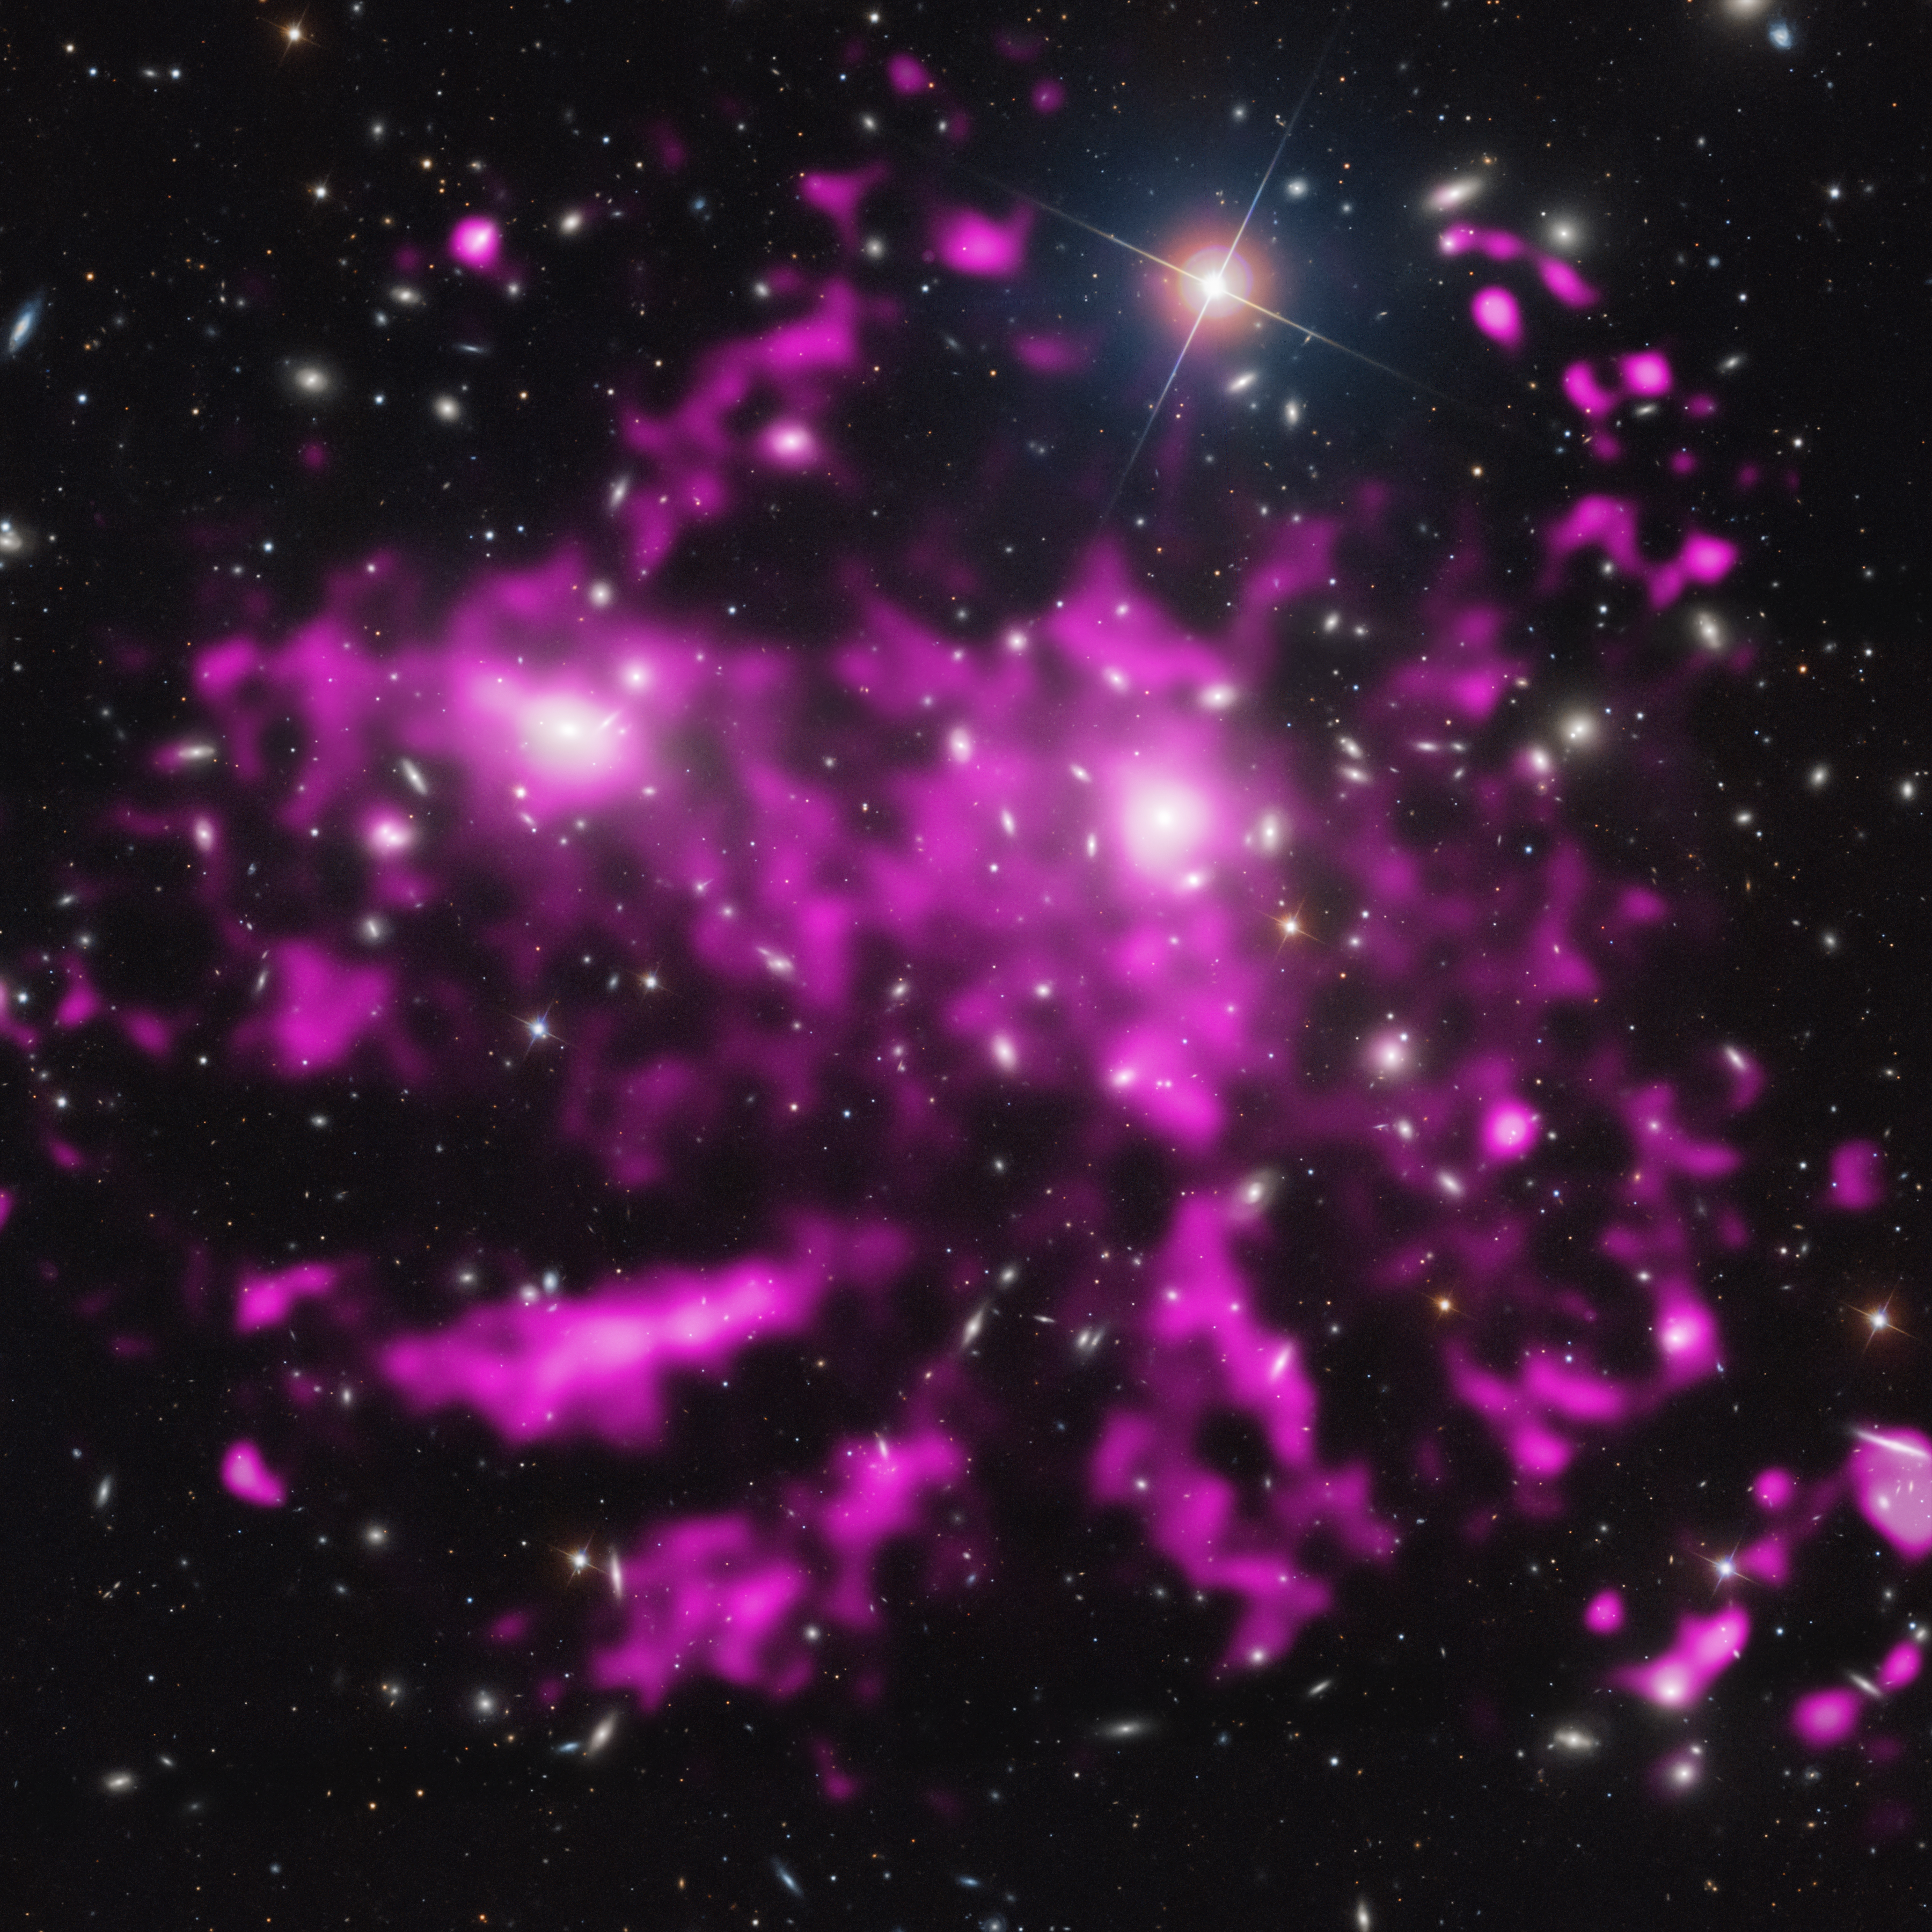
\includegraphics[width=8cm]{coma_composite}
\centering
\caption{A composite image combining an X-ray data, courtesy of Chandra, and optical data, courtesy of the Sloan Digital Sky Survey.  Image credit: X-ray - NASA/CXC/MPE/J.Sanders et al, Optical - SDSS}
\end{figure}
	
	
\subsection{Dynamical Constraints from Galactic Rotation Curves}	
	
\href{http://www.skyandtelescope.com/astronomy-resources/vera-rubin-dark-matter-detective/}{summary source}	

\href{http://articles.adsabs.harvard.edu/full/1970ApJ...159..379R}{rubin paper source}	
	
Nearly fourty years later, stronger evidence was provided for the existence of dark matter by Vera Rubin and Kent Ford in their 1970 paper looking at the rotation curve of the Andomeda Galaxy.  In this paper, Rubin used the H$\alpha$ lines to determine the orbital velocities of different stars in the galaxy.  Later measurements used the 21 cm hyperfine transition line to measure orbital velocities within other galaxies (Begeman et al, 1990, \href{http://adsabs.harvard.edu/full/1991MNRAS.249..523B}{begeman paper source}	).
	
	From simple Newtonian arguments, one gets the following description of the orbital velocity inside a galaxy:
	
\begin{equation}
v(r) = \sqrt{\frac{G M(r)}{r}}
\end{equation}	

In this equation, M(r) is the sum of the masses of all the gas and stars inside a given radius.  Given that most of the mass from luminous matter is concentrated at the center, one would expect that at large distances from the center of the galaxy, the orbital velocity would fall off as $v \propto r^{-1/2}$.

However, what is seen differs from this simple approximation drastically.  The figure below is taken from a later study but the results are similar to what Rubin and Ford saw deecades earlier: the asymptotic behavior of the orbital velocity is constant and does not show any polynomial roll-off.  By isolating the contributions from measurable mass densities (such as visible matter and gas), one can get an idea of the density distribution of dark matter in a galaxy.  From the figure below, one could asymtotically estimate that $M(r) \propto r$ which would imply that $\rho(r) \propto r^{-2}$.  One quickly realizes that this cannot be the true density since the mass of the galaxy diverges but approximates the density within an effective radius.

\begin{figure}[h]
\includegraphics[width=8cm]{ngc_6503_rotation_curve}
\centering
\caption{The rotation curve of the galaxy NGC 6503 broken down into individual components: visible matter (dashed), gas (dotted), and dark matter (dash dotted) (Begeman et al, 1990, \href{http://adsabs.harvard.edu/full/1991MNRAS.249..523B}{begeman paper source}	). }
\end{figure}


\subsection{Evidence from Graviational Lensing}	

Gravitational lensing is the distortion of light coming from a source due to the warping of spacetime from the presence of large amounts of matter or energy.  In practice, graviational lensing results in the deflection of the light as seen in the figure below.  In a gravitational lensing system, if we know the redshift (distance) of the source and the lense, we can estimate the gravitational field of the lensing system and hence its mass.

\begin{SCfigure}[\sidecaptionrelwidth][h]
	\centering
	\caption{A cartoon showing the deflection of light due to the warping of spacetime caused by the presence of a massive galaxy cluster.  Note that for very strong lensing, one expects multiple images of the source object and sometimes even an Einstein Ring around the lense. Image credit: NASA/ESA.}
	\includegraphics[width=0.5\textwidth]{gravitation_lensing_cartoon}
	\label{fig:gravitation_lensing_cartoon}
\end{SCfigure}

\begin{SCfigure}[\sidecaptionrelwidth][h]
	\centering
	\caption{In this optical image you see the massive MACS J1149.6+2223 cluster.  In the zoomed portion, you can actually see the same supernova, SN Refsdal, in four smaller images around a large galaxy within the cluster. Image credit: HST.}
	\includegraphics[width=0.5\textwidth]{einstein_cross}
\end{SCfigure}

Mass estimation via gravitational lensing in itself is very useful for finding large discrepancies in mass from known sources and true mass (the discrepancy being attributed to dark matter).  However, when combined with x-ray measurements, as seen in Fig. \ref{fig:bullet_cluster}, one gets even more interesting results.  Shown in Fig. \ref{fig:bullet_cluster} is the Bullet Cluster which actually consists of two colliding sub-clusters.  In the image, X-ray map from Chandra X-ray observatory is shown in magenta while the mass distribution from gravitation lensing is shown in blue.  


\end{document}
